\documentclass[11pt]{article}
\usepackage{graphicx}
\usepackage{amssymb}
\usepackage{color}

\textwidth = 6.5 in
\textheight = 9 in
\oddsidemargin = 0.0 in
\evensidemargin = 0.0 in
\topmargin = 0.0 in
\headheight = 0.0 in
\headsep = 0.0 in
\parskip = 0.2in
\parindent = 0.0in


\begin{document}
{\large {\bf CMPT 202 - Tree Exercises}} \\

Most of the following questions refer to the tree shown below:





\begin{figure}[h]

\centerline {
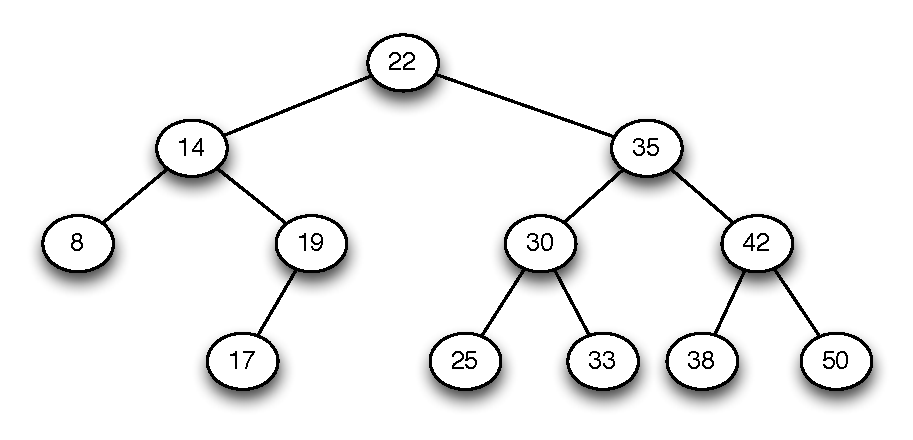
\includegraphics[width=5in]{TreeExerciseGraph.pdf}
}
%\caption{Example tree}
\label{fig:fig1}
\end{figure}

\begin{enumerate}

\item What node is at the root of the tree? {\color{red} }

\item What are the leaf nodes?

\item What node is the parent of 42?

\item Are nodes 19 and 30 siblings?

\item What is the height of this tree?

\item What level is node 19?

\item Is this a binary or general tree?

\item If it is a binary tree, is it

\begin{enumerate}

\item a binary search tree?

\item a full binary tree?

\item a complete binary tree?

\end{enumerate}

\item What are the pre-order, in-order, and post-order traversals of this tree?

\item {Write the expression tree for the following expressions: \\ \\
$m * n * o + p$ \hspace*{3in}$a * (b + c) * d$
}

\pagebreak
\item What is the height of the shortest binary tree that contains 21 nodes?

\item Draw the shortest possible binary search tree from the following set of strings 
\begin{center}\{ {\it Ann, Ben, Charles, David, Elizabeth, Fred, Gary, Harold, Isabel, Jay, Kelly} \}\end{center}

\item At most how many nodes can a binary tree have at level $n$?

\item Insert the following values into a binary search tree:
\begin{center} \{ 26, 12, 2, 3, 4, 5, 15, 35, 1 \} \end{center}

\item Show the resulting tree after deleting the node with value 35.

\item Provide three examples from everyday life where a decision tree can be used?

\end{enumerate}


 \end{document}
